\chapter{Ergebnisse}\label{chap:Ergebnisse}

In diesem Kapitel werden in \hyperref[sec:Hyperparameter]{Abschnitt 6.1} zunächst die Ergebnisse der Hyperparameteroptimierung und somit die jeweils optimale Hyperparameterkombination der Modelle vorgestellt. Anschließend werden die Modelle auf Daten der Quelldomäne (\hyperref[sec:quelldomäne]{Abschnitt 6.2}) und auf Daten der Zieldomäne (\hyperref[sec:zieldomäne]{Abschnitt 6.3}) evaluiert. Zuletzt werden in \hyperref[sec:nichtnormalisiert]{Abschnitt 6.4} Ergebnisse von Modellen, welche mit nicht-normalisierten Daten trainiert wurden, präsentiert.


\section{Ergebnisse der Hyperparameteroptimierung}\label{sec:Hyperparameter}

Die Hyperparameteroptimierungen wurde ausgewertet, indem für die Metriken der 5 Modelle der Cross Validation der Mittelwert gebildet und von diesem die Standardabweichung $\sigma$ zwischen den 5 Modellen abgezogen wurde. Die beste Hyperparameterkombination wurde anhand des F1-Scores ausgewählt.  Optimierte Hyperparameter sind Anzahl der Inception Module, genannt \texttt{depth d}, \texttt{learning rate l} und \texttt{batch size b}.

\begin{table}[h!]
\centering
\caption[Hyperparameteroptimierung des DANNs]{Ergebnisse der Grid Search für das \gls{DANN}. Optimierte Hyperparameter sind \texttt{depth d} (Anzahl der Inception Module), \texttt{learning rate l} und \texttt{batch size b}. Die Metriken wurden berechnet, indem vom Durchschnitt aus allen 5 Folds der Cross Validation die Standardabweichung $\sigma$ abgezogen wurde. $\sigma$ ist für die jeweilige Metrik rechts neben der betreffenden Metrik angegeben. Negative Werte kommen zustande, wenn $\sigma$ größer als der Durchschnitt ist. Die beste Hyperparameterkombination ist fett hervorgehoben. }
\label{tab:GridSearch_DANN}
\begin{tabular}{lcccccc}
\toprule
\textbf{Hyperparameterkombination} & \textbf{F1} & \textbf{$\sigma$} & \textbf{Recall} & \textbf{$\sigma$} & \textbf{Specificity} & \textbf{$\sigma$}\\
%depth learning rate batch size &&&&&&\\
\midrule 
d=3 l=0,0001 b=128  & 0,931  & 0,005  & 0,941  & 0,003 & 0,915 & 0,012 \\
d=3 l=0,0001 b=64  & 0,930  & 0,005  & 0,919  & 0,012 & 0,931 & 0,008 \\
d=3 l=0,0001 b=32  & 0,929  & 0,004  & 0,928  & 0,008 & 0,923 & 0,006 \\
d=3 l=0,001	b=128  & 0,369  & 0,303  & 0,312  & 0,365 & 0,650 & 0,206 \\
d=3 l=0,001	b=64  & 0,333  & 0,365  & 0,380  & 0,382 & 0,383 & 0,385 \\
d=3 l=0,001	b=32  & 0,765  & 0,113  & 0,921  & 0,005 & 0,439 & 0,335 \\
d=3 l=0,01 b=128  & -0,134  & 0,268  & -0,200  & 0,400 & 0,400 & 0,400 \\
d=3 l=0,01 b=64  & -0,134  & 0,268  & -0,200  & 0,400 & 0,400 & 0,400 \\
d=3 l=0,01 b=32  & -0,134  & 0,268  & -0,200  & 0,400 & 0,400 & 0,400 \\
d=6 l=0,0001 b=128  & 0,951  & 0,002  & 0,943  & 0,003 & 0,957 & 0,005 \\
d=6 l=0,0001 b=64  & 0,949  & 0,003  & 0,935  & 0,007 & 0,959 & 0,005 \\
d=6 l=0,0001 b=32  & 0,950  & 0,003  & 0,943  & 0,005 & 0,953 & 0,007 \\
d=6 l=0,001 b=128  & 0,950  & 0,003  & 0,939  & 0,005 & 0,962 & 0,003 \\
d=6 l=0,001 b=64  & 0,387  & 0,377  & 0,380  & 0,374 & 0,959 & 0,012 \\
d=6 l=0,001 b=32  & 0,381  & 0,381  & 0,377  & 0,377 & 0,956 & 0,016 \\
d=6 l=0,01 b=128  & -0,134  & 0,268  & -0,200  & 0,400 & 0,400 & 0,400 \\
d=6 l=0,01 b=64  & -0,134  & 0,268  & -0,200  & 0,400 & 0,400 & 0,400 \\
d=6 l=0,01 b=32  & -0,134  & 0,268  & -0,200  & 0,400 & 0,400 & 0,400 \\
d=9 l=0,0001 b=128  & 0,952  & 0,003  & 0,940  & 0,005 & 0,959 & 0,008 \\
d=9 l=0,0001 b=64  & 0,952  & 0,003  & 0,940  & 0,007 & 0,961 & 0,005 \\
\textbf{d=9 l=0,0001 b=32}  & \textbf{0,954}  & \textbf{0,002}  & \textbf{0,943}  & \textbf{0,004} & \textbf{0,964} & \textbf{0,003} \\
d=9 l=0,001 b=128  & 0,952  & 0,001  & 0,944  & 0,003 & 0,958 & 0,004 \\
d=9 l=0,001 b=64  & 0,954  & 0,002  & 0,945  & 0,004 & 0,958 & 0,004 \\
d=9 l=0,001 b=32  & 0,950  & 0,002  & 0,937  & 0,006 & 0,961 & 0,003 \\
d=9 l=0,01 b=128  & -0,083  & 0,406  & -0,088  & 0,476 & 0,395 & 0,396 \\
d=9 l=0,01 b=64  & -0,134  & 0,268  & -0,200  & 0,400 & 0,400 & 0,400 \\
d=9 l=0,01 b=32  & -0,134  & 0,268  & -0,200  & 0,400 & 0,400 & 0,400 \\

\bottomrule
\end{tabular}
\end{table}

\subsection*{DANN}

Alle Hyperparameterkombinationen und deren Klassifikationsgüte sind in \hyperref[tab:GridSearch_DANN]{Tab.~6.1} zu sehen. Die beste Hyperparameterkombination ist diejenige mit 9 Inception Modulen, einer \texttt{learning rate} von 0,0001 und einer \texttt{batch size} von 32. Sie erreicht einen F1-Score von 0,954 (Mittelwert - $\sigma$), einen Recall von 0,943 (Mittelwert - $\sigma$) und eine Specificity von 0,964 (Mittelwert - $\sigma$).
In \hyperref[fig:DANN_training]{Abb.~6.1} ist als Beispiel der Trainings- und Validierungsverlauf von Loss und Accuracy des Label Predictors und des Domain Classifiers des \gls{DANN} Modells aus Fold 1 der Cross Validation zu sehen. 

\begin{figure}[!ht]%
\centering
	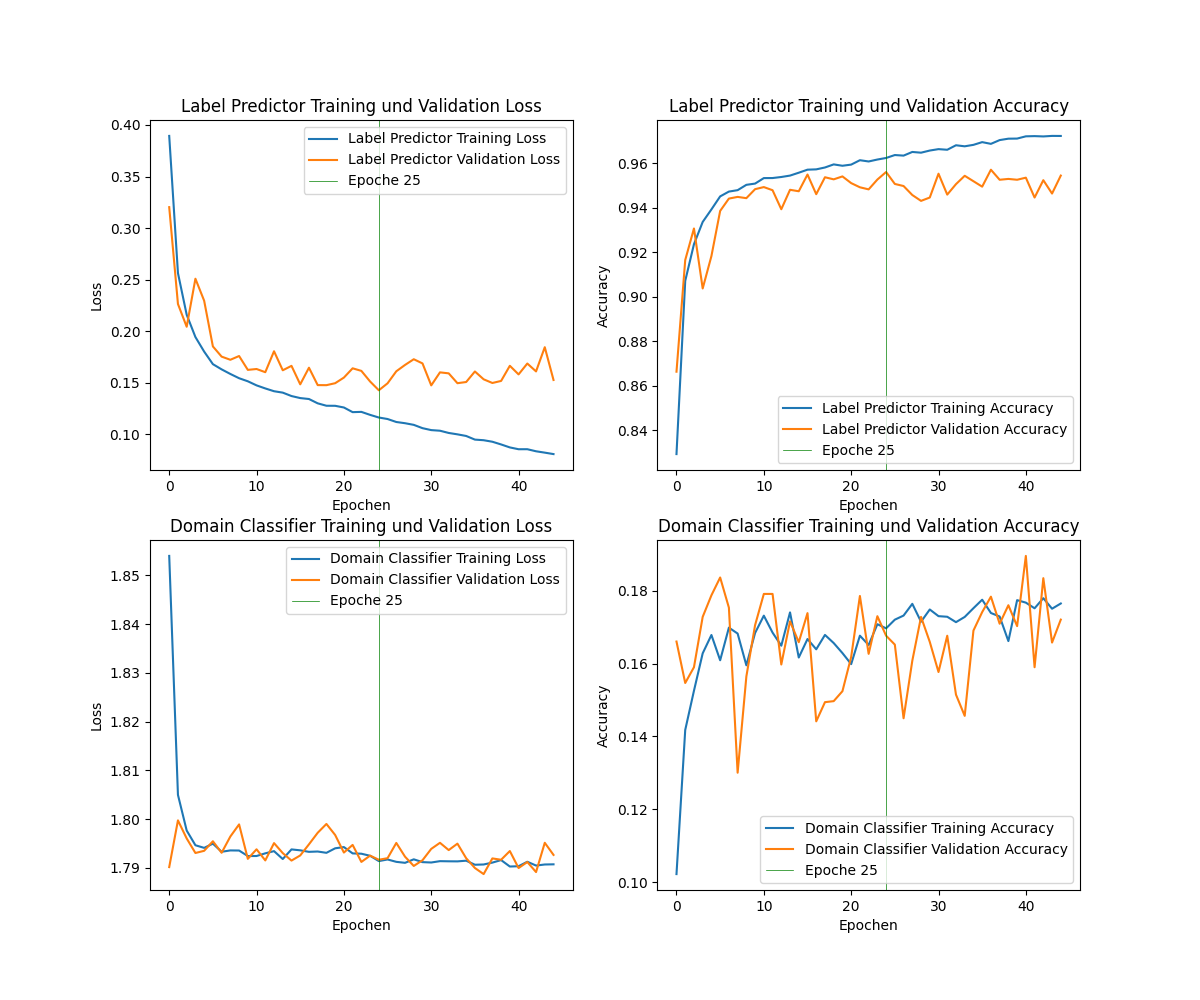
\includegraphics[width=1\textwidth]{./Bilder/DANN_training_fold1.png}
\caption[DANN Training Plots]{Trainings- und Validierungsverlauf des Label Predictors (oben) und des Domain Classifiers (unten) des \gls{DANN} Modells aus Fold 1 der Cross Validation. Epoche 25 ist die beste Epoche des Trainings.} 
\label{fig:DANN_training}
\end{figure} 

\subsection*{DANNdirect}

Für das \gls{DANN}direct wurde keine separate Grid Search durchgeführt, sondern es wurde diejenige Hyperparameterkombination für das Training genutzt, die bei der Grid Search des \gls{DANN} als am besten identifiziert wurde. Es erreicht mit 9 Inception Modulen, einer \texttt{learning rate} von 0,0001 und einer \texttt{batch size} von 32 einen F1-Score von 0,937 (bereinigt um $\sigma$ = 0,003), einen Recall von 0,932 (bereinigt um $\sigma$ = 0,009) und eine Specificity von 0,933 (bereinigt um $\sigma$ = 0,007). 

\subsection*{Vergleichsmodell InceptionTime}

Die vollständigen Ergebnisse der Grid Search des InceptionTime Modells sind im \hyperref[tab:GridSearch_InceptionTime]{Anhang A.1} zu finden. Die beste Hyperparameterkombination ist diejenige mit 9 Inception Modulen, einer \texttt{learning rate} von 0,0001 und einer \texttt{batch size} von 64. Die durchschnittlichen Werte der Modelle aus der Cross Validation sind ein F1-Score von 0,939 (bereinigt um $\sigma$ = 0,002), einen Recall von 0,935 (bereinigt um $\sigma$ = 0,006) und eine Specificity von 0,939 (bereinigt um $\sigma$ = 0,003).

\begin{table}[h!]
\centering
\caption[Ergebnisse der Evaluation auf der Quelldomäne xECGArch]{Evaluation der Modelle mit dem Testdatensatz der xECGArch-Datenbank. Globaler F1-Score der gewichteten und ungewichteten Ensembles, sowie Standardabweichung $\sigma$ und Durchschnittswert der Einzelmodelle. Der beste Wert ist hervorgehoben.}
\label{tab:Ergebnisse_indomain}
\begin{tabular}{lccccc}
\toprule
\textbf{Modell}       & \multicolumn{4}{c}{\textbf{xECGArch-Datenbank}} \\ 
\cmidrule(lr){2-5}
					  & \textbf{\makecell{F1 $\varnothing$ Modelle}} & \textbf{\makecell{$\sigma$}} & \textbf{\makecell{F1 Ensemble\\ gewichtet}} & \textbf{\makecell{F1 Ensemble\\ ungewichtet}} \\ \hline
\textbf{DANN} 			& 0,947           & 0,003            & \textbf{0,951}             & 0,950                   \\
\textbf{DANNdirect}     & 0,931           & 0,003            & 0,940             & 0,938 
\\
\textbf{InceptionTime}  & 0,930           & 0,002            & 0,938             & 0,938 
\\
\bottomrule
\end{tabular}
\end{table}

\section{Evaluierung auf Daten der Quelldomäne}\label{sec:quelldomäne}

\begin{table}[h!]
\centering
\caption[Ergebnisse der Evaluation auf der Quelldomäne xECGArch pro Ableitung]{Evaluation der Modelle mit dem Testdatensatz der xECGArch-Datenbank. Ergebnisse des gewichteten und ungewichteten Ensembles. Der jeweils beste F1-Score pro Ableitung ist hervorgehoben. }
\label{tab:Ergebnisse_indomain_leads}
\begin{tabular}{lccccccc}
\toprule
\textbf{Modell}     & \multicolumn{3}{c}{\textbf{Ensemble gewichtet}} & \multicolumn{3}{c}{\textbf{Ensemble ungewichtet}}\\
						& \textbf{F1} & \textbf{Recall} & \textbf{Specificity} & \textbf{F1} & \textbf{Recall} & \textbf{Specificity}\\  
\midrule
					   & \multicolumn{6}{c}{{Ableitung I}} \\ 
\cmidrule(lr){2-7}
\textbf{DANN} 			& \textbf{0,947}  & 0,933  & 0,960 & 0,945 & 0,935 & 0,954 \\
\textbf{DANNdirect}     & 0,931  & 0,935  & 0,923 & 0,928 & 0,931 & 0,921 \\
\textbf{InceptionTime}  & 0,929  & 0,929  & 0,925 & 0,930 & 0,931 & 0,925 \\
\midrule
					   & \multicolumn{6}{c}{{Ableitung II}} \\ 
\cmidrule(lr){2-7}
\textbf{DANN} 			& \textbf{0,954}  & 0,933  & 0,975 & \textbf{0,954} & 0,933 & 0,975 \\
\textbf{DANNdirect}     & 0,947  & 0,943  & 0,950 & 0,941 & 0,931 & 0,952 \\
\textbf{InceptionTime}  & 0,946  & 0,941  & 0,950 & 0,946 & 0,937 & 0,954 \\
\midrule
					   & \multicolumn{6}{c}{{ Ableitung III}} \\ 
\cmidrule(lr){2-7}
\textbf{DANN} 			& \textbf{0,946}  & 0,929  & 0,962 & 0,943 & 0,923 & 0,962 \\
\textbf{DANNdirect}     & 0,939  & 0,937  & 0,937 & 0,937 & 0,937 & 0,933 \\
\textbf{InceptionTime}  & 0,935  & 0,929  & 0,939 & 0,935 & 0,929 & 0,939 \\
\midrule
					   & \multicolumn{6}{c}{{ Ableitung aVR}} \\ 
\cmidrule(lr){2-7}
\textbf{DANN} 			& \textbf{0,962}  & 0,955  & 0,969 & 0,961 & 0,951 & 0,971 \\
\textbf{DANNdirect}     & 0,944  & 0,939  & 0,948 & 0,942 & 0,935 & 0,948 \\
\textbf{InceptionTime}  & 0,943  & 0,937  & 0,948 & 0,943 & 0,933 & 0,952 \\
\midrule
					   & \multicolumn{6}{c}{{ Ableitung aVL}} \\ 
\cmidrule(lr){2-7}
\textbf{DANN} 			& \textbf{0,944}  & 0,931  & 0,956 & 0,943 & 0,927 & 0,958 \\
\textbf{DANNdirect}     & 0,930  & 0,935  & 0,921 & 0,926 & 0,929 & 0,919 \\
\textbf{InceptionTime}  & 0,926  & 0,929  & 0,919 & 0,921 & 0,925 & 0,910 \\
\midrule
					   & \multicolumn{6}{c}{{ Ableitung aVF}} \\ 
\cmidrule(lr){2-7}
\textbf{DANN} 			& 0,956  & 0,939  & 0,973  & \textbf{0,957} & 0,941 & 0,973 \\
\textbf{DANNdirect}     & 0,950  & 0,945  & 0,952  & 0,953 & 0,949 & 0,956 \\
\textbf{InceptionTime}  & 0,950  & 0,949  & 0,948  & 0,950 & 0,947 & 0,952\\
\bottomrule
\end{tabular}
\end{table}


Die Modelle wurden auf dem Testdatensatz der xECGArch-Datenbank evaluiert. Auf diesen Datensatz hatten die Modelle während des Trainings keinen Zugriff. Zur Klassifikation wurden für alle \gls{EKG}s die Ableitungen I, II, III, aVR, aVL und aVF als eine gemischte Datenmenge eingegeben, analog zur Struktur des Trainingsdatensatzes. Der globale F1-Score wurde aus der Gesamtmenge der Vorhersagen gesammelt berechnet. Das dynamisch nach Klassifikationssicherheit der einzelnen Modelle gewichtete \gls{DANN} Ensemble erreicht mit 0,951 den besten globalen F1-Score. Die globalen F1-Scores der Ensembles, sowie den Durchschnitt der einzelnen Modelle der Ensembles und die Standardabweichung dieser lassen sich in \hyperref[tab:Ergebnisse_indomain]{Tab.~6.2} nachlesen. 

In den Abbildungen \hyperref[fig:DANN_label_roc]{6.2} und \hyperref[fig:DANN_label_roc]{6.3} sind als Beispiel die \gls{ROC}-Kurven des Label Predictors und des Domain Classifiers des \gls{DANN} Modells aus Fold 1 der Cross Validation dargestellt. Dabei fällt auf, dass die ROC-Kurve des Label Predictors des \gls{DANN} Modells eine große Fläche von 0,982 aufspannt, während die ROC-Kurven des Domain Classifiers des \gls{DANN} Modells nahe an der Winkelhalbierenden liegen und Flächen zwischen 0,477 bis 0,564 aufspannen.

Aufgeteilt nach Ableitung (siehe \hyperref[tab:Ergebnisse_indomain_leads]{Tab.~6.3}) wird der beste F1-Score mit 0,962 auf Ableitung aVR vom gewichteten \gls{DANN} Ensemble erreicht. Die durchschnittlichen F1-Scores der Ensembles über alle Ableitungen betragen für das \gls{DANN} 0,952 im gewichteten und 0,951 im ungewichteten Fall. Das gewichtete DANNdirect Ensemble erreicht einen durchschnittlichen F1-Score von 0,940 und das ungewichtete einen von 0,938. Das gewichtete und ungewichtete InceptionTime Ensemble erreichen einen durchschnittlichen F1-Score von 0,938. 



\begin{figure}[!ht]%
\centering
	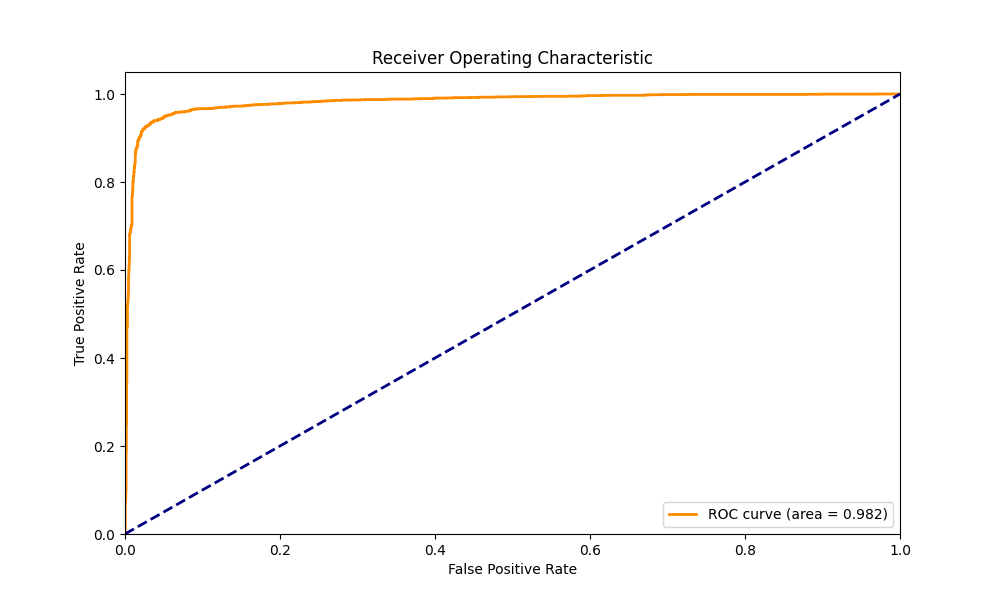
\includegraphics[width=0.8\textwidth]{./Bilder/DANN_roc_label_fold1.png}
\caption[Label Predictor ROC-Kurve]{Receiver-Operating-Characteristic-Kurve des Label Predictors des \gls{DANN} Modells aus Fold 1 der Cross Validation.} 
\label{fig:DANN_label_roc}
\end{figure}

\begin{figure}[!ht]%
\centering
	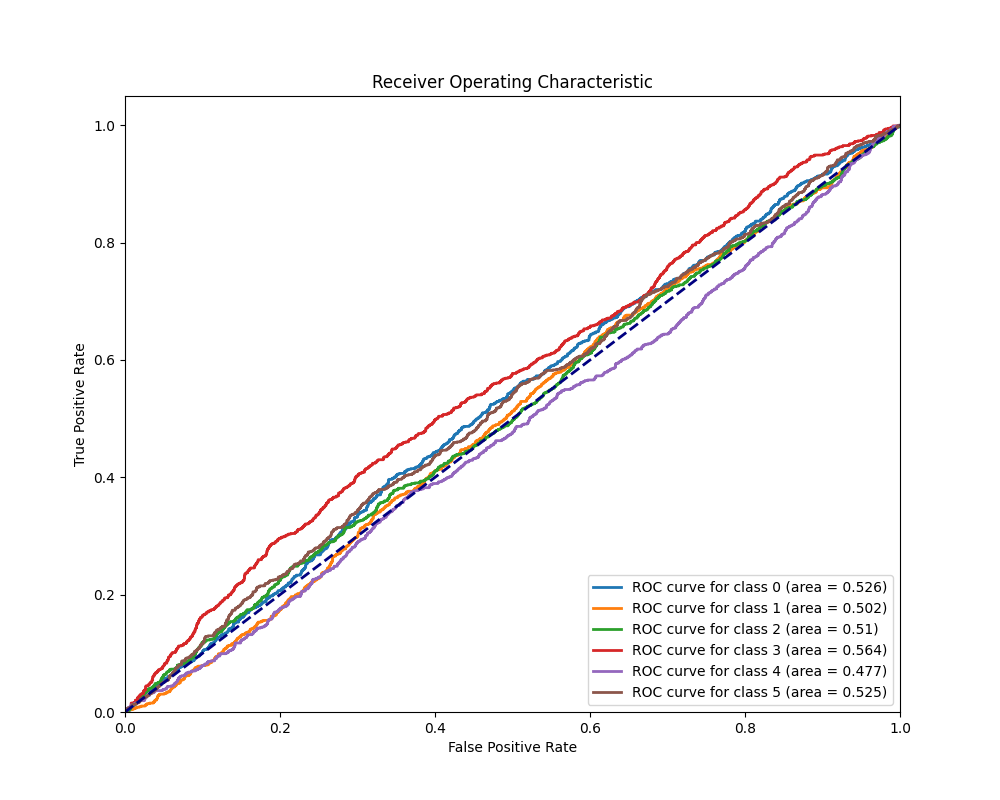
\includegraphics[width=0.8\textwidth]{./Bilder/DANN_roc_domain_fold1.png}
\caption[Domain Classifier ROC-Kurven]{Receiver-Operating-Characteristic-Kurve des Domain Classifiers des \gls{DANN} Modells aus Fold 1 der Cross Validation. } 
\label{fig:DANN_label_roc}
\end{figure}



\section{Evaluierung auf Daten der Zieldomänen}\label{sec:zieldomäne}

Um einzuschätzen, wie die Modelle mit einem Domain Shift umgehen, wurden die Modelle auf Daten von mobilen \gls{EKG}-Patches evaluiert, deren Signale eine andere Morphologie im Vergleich zu 12-Kanal-\gls{EKG}-Signalen aufweisen.

\subsubsection*{Icentia11k}

Bei der Icentia11k-Datenbank erreicht das ungewichtete \gls{DANN} Ensemble mit 0,666 den besten F1-Score (siehe \hyperref[tab:Ergebnisse_Icentia11k]{Tab.~6.4}) und den besten Recall mit 0,979. Die beste Specificity wird mit 0,952 sowohl vom ungewichteten als auch vom gewichteten \gls{DANN} Ensemble erreicht (siehe \hyperref[tab:sens_icentia]{Tab.~6.5}).

\begin{table}[h!]
\centering
\caption[Ergebnisse der Evaluation auf der Zieldomäne Icentia11k]{Evaluation der Modelle auf der Zieldomäne Icentia11k. F1-Score der gewichteten und ungewichteten Ensembles, sowie Standardabweichung $\sigma$ und Durchschnittswert der Einzelmodelle.}
\label{tab:Ergebnisse_Icentia11k}
\begin{tabular}{lccccc}
\toprule
\textbf{Modell}       & \multicolumn{4}{c}{\textbf{Icentia11k}} \\ 
\cmidrule(lr){2-5}
					  &\textbf{\makecell{F1 $\varnothing$ Modelle}} & \textbf{\makecell{$\sigma$}} & \textbf{\makecell{F1 Ensemble\\gewichtet}} & \textbf{\makecell{F1 Ensemble\\ungewichtet}} \\ \hline
\textbf{DANN} 			& 0,641           & 0,018            & 0,665             & \textbf{0,666}                   \\
\textbf{DANNdirect}     & 0,498           & 0,032            & 0,518             & 0,515 
\\
\textbf{InceptionTime}  & 0,520           & 0,013            & 0,543             & 0,541 
\\
\bottomrule
\end{tabular}
\end{table}


\begin{table}[h!]
\centering
\caption[Recall und Specificity Icentia11k]{Evaluation der Modelle auf der Zieldomäne Icentia11k. Recall und Specificity des gewichteten und ungewichteten Ensembles. }
\label{tab:sens_icentia}
\begin{tabular}{lccccc}
\toprule
\textbf{Modell}     & \multicolumn{2}{c}{\textbf{Ensemble gewichtet}} & \multicolumn{2}{c}{\textbf{Ensemble ungewichtet}}\\
						& \textbf{Recall} & \textbf{Specificity}  & \textbf{Recall} & \textbf{Specificity}\\  
\midrule
%					   & \multicolumn{4}{c}{{Ableitung 1}} \\ 
%\cmidrule(lr){2-5}
\textbf{DANN} 			& 0,973  & 0,952  & 0,979 & 0,952  \\
\textbf{DANNdirect}     & 0,947  & 0,915  & 0,943 & 0,915  \\
\textbf{InceptionTime}  & 0,936  & 0,925  & 0,936 & 0,924  \\

\bottomrule
\end{tabular}
\end{table}

\subsubsection*{TIMELY-Datensatz}

Die durchschnittliche Klassifikationsgüte der Ensembles auf dem TIMELY-Datensatz beträgt für das \gls{DANN} 0,973 (F1-Score) im gewichteten und 0,969 (F1-Score) im ungewichteten Fall. Das gewichtete DANNdirect Ensemble erreicht einen durchschnittlichen F1-Score von 0,948 und das ungewichtete einen von 0,947. Das gewichtete und das ungewichtete InceptionTime Ensemble erreichen jeweils einen durchschnittlichen F1-Score von 0,949.

Die Ergebnisse des TIMELY-Datensatzes wurden nach Ableitung aufgeschlüsselt. Auf allen drei Ableitungen erreicht jeweils das gewichtete \gls{DANN} Ensemble den besten F1-Score mit 0,952 auf Ableitung 1, 0,986 auf Ableitung 2 und 0,981 auf Ableitung 3 (siehe \hyperref[tab:Ergebnisse_timely]{Tab.~6.6}). Recall und Specificity der Modelle lässt sich aus \hyperref[tab:sens_timely]{Tab.~6.7} entnehmen.

\begin{table}[h!]
\centering
\caption[Ergebnisse der Evaluation auf der Zieldomäne TIMELY]{Evaluation der Modelle mit den drei Ableitungen des TIMELY-Datensatzes. F1-Score der gewichteten und ungewichteten Ensembles, sowie Standardabweichung $\sigma$ und Durchschnittswert der Einzelmodelle.}
\label{tab:Ergebnisse_timely}
\begin{tabular}{lccccc}
\toprule
\textbf{Modell}   & \textbf{\makecell{F1 $\varnothing$ Modelle}} & \textbf{\makecell{$\sigma$}} & \textbf{\makecell{F1 Ensemble\\gewichtet}} & \textbf{\makecell{F1 Ensemble\\ungewichtet}} \\     
			  
\midrule
 & \multicolumn{4}{c}{{TIMELY Ableitung 1}} \\   
\cmidrule(lr){2-5}
					  
\textbf{DANN} 			& 0,946           & 0,022            & \textbf{0,952}             & 0,942                   \\
\textbf{DANNdirect}     & 0,908           & 0,020            & 0,903             & 0,905 
\\
\textbf{InceptionTime}  & 0,908           & 0,026            & 0,904             & 0,905 
\\
\midrule

 		& \multicolumn{4}{c}{{TIMELY Ableitung 2}} \\ 
\cmidrule(lr){2-5}

\textbf{DANN} 			& 0,972           & 0,022            & \textbf{0,986}             & 0,985                   \\
\textbf{DANNdirect}     & 0,969           & 0,004            & 0,972             & 0,972 
\\
\textbf{InceptionTime}  & 0,971           & 0,004            & 0,976             & 0,975 
\\
\midrule
       & \multicolumn{4}{c}{{TIMELY Ableitung 3}} \\ 
\cmidrule(lr){2-5}

\textbf{DANN} 			& 0,972           & 0,006            & \textbf{0,981}             & 0,980                   \\
\textbf{DANNdirect}     & 0,959           & 0,005            & 0,969             & 0,965 
\\
\textbf{InceptionTime}  & 0,957           & 0,006            & 0,968             & 0,968 
\\
\bottomrule
\end{tabular}
\end{table}


\begin{table}[h!]
\centering
\caption[Recall und Specificity TIMELY]{Evaluation der Modelle auf der Zieldomäne TIMELY. Recall und Specificity des gewichteten und ungewichteten Ensembles. }
\label{tab:sens_timely}
\begin{tabular}{lccccc}
\toprule
\textbf{Modell}     & \multicolumn{2}{c}{\textbf{Ensemble gewichtet}} & \multicolumn{2}{c}{\textbf{Ensemble ungewichtet}}\\
						& \textbf{Recall} & \textbf{Specificity}  & \textbf{Recall} & \textbf{Specificity}\\  
\midrule
					   & \multicolumn{4}{c}{{TIMELY Ableitung 1}} \\ 
\cmidrule(lr){2-5}
\textbf{DANN} 			& 1,00  & 0,927  & 1,00 & 0,912  \\
\textbf{DANNdirect}     & 0,997  & 0,848  & 0,995 & 0,853  \\
\textbf{InceptionTime}  & 0,998  & 0,850  & 0,998 & 0,851  \\
\midrule
					   & \multicolumn{4}{c}{{TIMELY Ableitung 2}} \\ 
\cmidrule(lr){2-5}
\textbf{DANN} 			& 1,00  & 0,979  & 1,00 & 0,978  \\
\textbf{DANNdirect}     & 0,981  & 0,973  & 0,981 & 0,972  \\
\textbf{InceptionTime}  & 0,981  & 0,979  & 0,981 & 0,978  \\
\midrule
					   & \multicolumn{4}{c}{{TIMELY Ableitung 3}} \\ 
\cmidrule(lr){2-5}
\textbf{DANN} 			& 1,00  & 0,971  & 1,00 & 0,969  \\
\textbf{DANNdirect}     & 0,977  & 0,971  & 0,974 & 0,967  \\
\textbf{InceptionTime}  & 0,978  & 0,969  & 0,980 & 0,967  \\

\bottomrule
\end{tabular}
\end{table}

\subsubsection*{SHDB-AF}

Da 23 Patienten der \gls{SHDB-AF} während ihrer Aufnahme keine \gls{VHF}-Episode hatten, konnte für diese Patienten der Recall und somit der F1-Score nicht berechnet werden, sodass die Evaluierung nur für die übrigen 77 Patienten durchgeführt wurde. 
Bei der \gls{SHDB-AF} erreicht das \gls{DANN} Ensemble einen durchschnittlichen F1-Score von 0,815 im gewichteten und einen durchschnittlichen F1-Score von 0,810 im ungewichteten Fall. Das gewichtete DANNdirect Ensemble erreicht einen durchschnittlichen F1-Score von 0,755 und das ungewichtete einen durchschnittlichen F1-Score von 0,753. Für das gewichtete InceptionTime Ensemble beträgt der durchschnittliche F1-Score 0,757 und für das ungewichtete beträgt der durchschnittliche F1-Score 0,756.
Die Standardabweichung im F1-Score des gewichteten \gls{DANN} Ensembles zwischen den 77 Patienten mit \gls{VHF} beträgt 0,220.



In \hyperref[tab:Ergebnisse_shdb]{Tab.~6.8} und \hyperref[tab:sens_shdb]{Tab.~6.9} ist die Klassifikationsgüte der Modelle nach Ableitung aufgeschlüsselt. Auf den einzelnen Ableitungen erreicht das gewichtete \gls{DANN} den besten F1-Score mit 0,777 auf der CC5-Ableitung und 0,852 auf der NASA-Ableitung. 


\begin{table}[h!]
\centering
\caption[Ergebnisse der Evaluation auf der Zieldomäne SHDB-AF]{Evaluation der Modelle mit den zwei Ableitungen der SHDB-AF-Datenbank. F1-Score der gewichteten und ungewichteten Ensembles, sowie Standardabweichung $\sigma$ und Durchschnittswert der Einzelmodelle.}
\label{tab:Ergebnisse_shdb}
\begin{tabular}{lccccc}
\toprule
\textbf{Modell} & \textbf{\makecell{F1 $\varnothing$ Modelle}} & \textbf{\makecell{$\sigma$}} & \textbf{\makecell{F1 Ensemble\\gewichtet}} & \textbf{\makecell{F1 Ensemble\\ungewichtet}} \\   
\midrule
					& \multicolumn{4}{c}{{SHDB-AF CC5-Ableitung}} \\ 
\cmidrule(lr){2-5}
\textbf{DANN} 			& 0,763           & 0,014            & \textbf{0,777}             & 0,776                   \\
\textbf{DANNdirect}     & 0,694           & 0,028            & 0,717             & 0,715 
\\
\textbf{InceptionTime}  & 0,717           & 0,012            & 0,731             & 0,730 
\\
\midrule
       & \multicolumn{4}{c}{{SHDB-AF NASA-Ableitung}} \\ 
\cmidrule(lr){2-5}
	
\textbf{DANN} 			& 0,824           & 0,012            & \textbf{0,852}             & 0,844                   \\
\textbf{DANNdirect}     & 0,753           & 0,018            & 0,793             & 0,790 
\\
\textbf{InceptionTime}  & 0,753           & 0,012            & 0,783             & 0,781 
\\
\bottomrule
\end{tabular}
\end{table}



\begin{table}[h!]
\centering
\caption[Recall und Specificity SHDB-AF]{Evaluation der Modelle auf der Zieldomäne \gls{SHDB-AF}. Recall und Specificity des gewichteten und ungewichteten Ensembles. }
\label{tab:sens_shdb}
\begin{tabular}{lccccc}
\toprule
\textbf{Modell}     & \multicolumn{2}{c}{\textbf{Ensemble gewichtet}} & \multicolumn{2}{c}{\textbf{Ensemble ungewichtet}}\\
						& \textbf{Recall} & \textbf{Specificity}  & \textbf{Recall} & \textbf{Specificity}\\  
\midrule
					   & \multicolumn{4}{c}{{CC5-Ableitung}} \\ 
\cmidrule(lr){2-5}
\textbf{DANN} 			& 0,949  & 0,947  & 0,949 & 0,947  \\
\textbf{DANNdirect}     & 0,948  & 0,904  & 0,946 & 0,903  \\
\textbf{InceptionTime}  & 0,951  & 0,912  & 0,948 & 0,914  \\
\midrule
					   & \multicolumn{4}{c}{{NASA-Ableitung}} \\ 
\cmidrule(lr){2-5}
\textbf{DANN} 			& 0,933  & 0,944  & 0,932 & 0,944  \\
\textbf{DANNdirect}     & 0,925  & 0,916  & 0,922 & 0,915  \\
\textbf{InceptionTime}  & 0,920  & 0,920  & 0,918 & 0,920  \\

\bottomrule
\end{tabular}
\end{table}

\section{Untersuchung des Einflusses der Normalisierung der Daten }\label{sec:nichtnormalisiert}

Im Rahmen dieser Arbeit wurden ebenfalls Modelle trainiert, ohne zuvor die Trainingsdaten zu z-normalisieren. Die beste Hyperparameterkombination dieser Modelle wurde ebenfalls per Grid Search ermittelt. Für das \gls{DANN} wurde als optimale Hyperparameterkombination 9 Inception Module, eine \texttt{learning rate} von 0,0001 und eine \texttt{batch size} von 64 ermittelt. Der durchschnittliche F1-Score abzüglich der Standardabweichung aus den Modellen der Cross Validation beträgt 0,956. Die Standardabweichung beträgt 0,002. Das DANNdirect wurde anschließend mit derselben Hyperparameterkombination trainiert.

Für InceptionTime wurde als optimale Hyperparameterkombination eine Anzahl von 9 Inception Modulen, eine \texttt{learning rate} von 0,001 und eine \texttt{batch size} von 128 ermittelt. Der durchschnittliche F1-Score abzüglich der Standardabweichung der InceptionTime Modelle aus der Cross Validation beträgt 0,941. Die Standardabweichung beträgt 0,003. 

Die Modelle wurden auf dem nicht normalisierten xECGArch-Testdatensatz evaluiert. Die höchste Klassifikationsgüte erreichen das gewichtete und ungewichtete \gls{DANN} Ensemble mit einem globalen F1-Score von 0,953 (siehe \hyperref[tab:Ergebnisse_indomain_notnorm]{Tab.~6.10}). Anschließend wurden die Modelle auf dem nicht-normalisierten TIMELY-Datensatz angewendet, um zu evaluieren, wie sie sich bei einem Domain Shift verhalten. In \hyperref[tab:Ergebnisse_timely_notnorm]{Tab.~6.11} ist die Klassifikationsgüte der Modelle für jede Ableitung des Datensatzes eingetragen. Die durchschnittlich höchste Klassifikationsgüte erreicht das \gls{DANN} Ensemble mit einem F1-Score von 0,946. 

\begin{table}[h!]
\centering
\caption[Ergebnisse der Evaluation auf der Quelldomäne mit nicht-normalisierten Daten]{Evaluation der Modelle mit dem nicht-normalisierten Testdatensatz der xECGArch-Datenbank. Globaler F1-Score der gewichteten und ungewichteten Ensembles, sowie Standardabweichung $\sigma$ und Durchschnittswert der Einzelmodelle. Der beste Wert ist hervorgehoben.}
\label{tab:Ergebnisse_indomain_notnorm}
\begin{tabular}{lccccc}
\toprule
\textbf{Modell}       & \multicolumn{4}{c}{\textbf{xECGArch-Datenbank}} \\ 
\cmidrule(lr){2-5}
					  & \textbf{\makecell{F1 $\varnothing$ Modelle}} & \textbf{\makecell{$\sigma$}} & \textbf{\makecell{F1 Ensemble\\ gewichtet}} & \textbf{\makecell{F1 Ensemble\\ ungewichtet}} \\ \hline
\textbf{DANN} 			& 0,948  & 0,003  & \textbf{0,953}  & \textbf{0,953}   \\
\textbf{DANNdirect}     & 0,932  & 0,003  & 0,937  & 0,938 \\
\textbf{InceptionTime}  & 0,934  & 0,003  & 0,942  & 0,942 \\
\bottomrule
\end{tabular}
\end{table}

\begin{table}[h!]
\centering
\caption[Ergebnisse der Evaluation auf nicht-normalisierten TIMELY-Daten]{Evaluation der Modelle mit den drei nicht-normalisierten Ableitungen des TIMELY-Datensatzes. F1-Score der gewichteten und ungewichteten Ensembles, sowie Standardabweichung $\sigma$ und Durchschnittswert der Einzelmodelle.}
\label{tab:Ergebnisse_timely_notnorm}
\begin{tabular}{lccccc}
\toprule
\textbf{Modell}   & \textbf{\makecell{F1 $\varnothing$ Modelle}} & \textbf{\makecell{$\sigma$}} & \textbf{\makecell{F1 Ensemble\\gewichtet}} & \textbf{\makecell{F1 Ensemble\\ungewichtet}} \\     
			  
\midrule
 & \multicolumn{4}{c}{{TIMELY Ableitung 1}} \\   
\cmidrule(lr){2-5}
					  
\textbf{DANN} 			& 0,935 & 0,014 & \textbf{0,949} & 0,947  \\
\textbf{DANNdirect}     & 0,892 & 0,022 & 0,891 & 0,892 \\
\textbf{InceptionTime}  & 0,902 & 0,025 & 0,916 & 0,915 \\
\midrule

 		& \multicolumn{4}{c}{{TIMELY Ableitung 2}} \\ 
\cmidrule(lr){2-5}

\textbf{DANN} 			& 0,938  & 0,036    & 0,921  & 0,917  \\
\textbf{DANNdirect}     & 0,931  & 0,039   & 0,940   & 0,961 \\
\textbf{InceptionTime}  & 0,952  & 0,007    & \textbf{0,967}  & 0,966 \\
\midrule
       & \multicolumn{4}{c}{{TIMELY Ableitung 3}} \\ 
\cmidrule(lr){2-5}

\textbf{DANN} 			& 0,936  & 0,022   & \textbf{0,968}   & 0,962 \\
\textbf{DANNdirect}     & 0,920  & 0,023   & 0,949   & 0,945 \\
\textbf{InceptionTime}  & 0,903  & 0,022   & 0,936   & 0,931 \\
\bottomrule
\end{tabular}
\end{table}
